\documentclass[a4paper]{article}
\usepackage{url} 
\usepackage{geometry}
\usepackage{graphicx}
\usepackage[parfill]{parskip}
\usepackage{pgfplots}
\usepackage{pgfplotstable}
\pgfplotsset{compat=newest}
\usepgfplotslibrary{fillbetween}

\definecolor{printred}{RGB}{215,25,28}
\definecolor{printorange}{RGB}{253,174,97}
\definecolor{printyellow}{RGB}{255,255,191}
\definecolor{printgreen}{RGB}{145,180,130}
\definecolor{printblue}{RGB}{43,131,186}
\definecolor{printlilac}{RGB}{178,171,210}

\begin{document}
\begin{figure}[ht]
\pgfplotstableread[col sep=comma]{data/pstate_power_4_cores.csv}\pstatelavamdtable
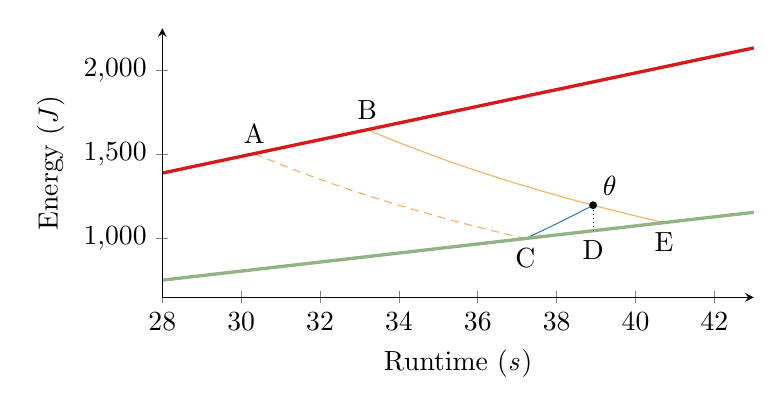
\begin{tikzpicture}
  \begin{axis}[
    axis on top,
    axis x line=bottom,
    axis y line=left,
    xlabel={Runtime (\emph{s})},
    ylabel={Energy (\emph{J})},    
    xmin=28, xmax=43,
    ymin=750, ymax=1874,
    ymin=650, ymax=2250,
    width=0.75\linewidth,
    height=5cm,
    legend columns=2,
    legend to name=leukocyte:legend,
    ]

    %% Model Parameters %%
    \pgfmathsetmacro{\baselinepower}{26.876067}
    \pgfmathsetmacro{\rooflinepower}{49.60612}
    \pgfmathsetmacro{\codepower}{30.775140866344813} 
    \pgfmathsetmacro{\codetime}{38.924663}
    \pgfmathsetmacro{\codeenergy}{1197.911987}
    \pgfmathsetmacro{\energyexp}{1.0}
    \pgfmathsetmacro{\timeexp}{2.0}

    % Sadly, pgfplots sucks too much to calculate cube roots
    % These values are calculated with a ruby script in tools
    \pgfmathsetmacro{\blnodex}{37.20603724152065}
    \pgfmathsetmacro{\brnodex}{40.72267572674299}
    \pgfmathsetmacro{\trnodex}{33.19809203308976}
    \pgfmathsetmacro{\tlnodex}{30.33124485283807}

    %% Intermezzo Values %%
    \pgfmathsetmacro{\brnodey}{\brnodex * \baselinepower}
    \pgfmathsetmacro{\blnodey}{\blnodex * \baselinepower}
    \pgfmathsetmacro{\tlnodey}{\tlnodex * \rooflinepower}
    \pgfmathsetmacro{\trnodey}{\trnodex * \rooflinepower}
    \pgfmathsetmacro{\codeenergy}{\codepower * \codetime}
    \pgfmathsetmacro{\baselineenergy}{\baselinepower * \codetime}

    % arguments: code power, code time, x - todo, apparently not supposed to do pgfmathparse
    \pgfmathdeclarefunction{metricbound}{3}{%
      \pgfmathparse{((#1 * #2^3) / #3^2)}%
    }
    \pgfmathdeclarefunction{definitionbound}{3}{%
      \pgfmathparse{((#1 / #2^3) * #3^4)}%
    }


    \addplot[color=printorange, forget plot, domain=\trnodex:\brnodex] { metricbound(\codepower, \codetime, x)};
    \addlegendimage{legend image with text={B\legendline{printorange}E}}
    \addlegendentry{Optimisation Bound}

    \addplot[color=printblue, forget plot, domain=\blnodex:\codetime] { definitionbound(\codepower, \codetime, x)};
    \addlegendimage{legend image with text={C\legendline{printblue}$\theta$}}
    \addlegendentry{Contribution Bound}

    \addplot[color=printorange, forget plot, densely dashed, domain=\tlnodex:\blnodex] {metricbound(\baselinepower, \blnodex, x)};
    \addlegendimage{legend image with text={A\legendline{printorange, densely dashed}C}}
    \addlegendentry{Optimisation Limit}

   % BETA ROOFLINE BOUND 
    \addplot[color=printred, very thick, domain=\pgfkeysvalueof{/pgfplots/xmin}:\pgfkeysvalueof{/pgfplots/xmax}] {\rooflinepower * x};
    \addlegendentry{$P_{max}$ Energy Bound}

    % ALPHA BASELINE BOUND 
    \addplot[color=printgreen, very thick, domain=\pgfkeysvalueof{/pgfplots/xmin}:\pgfkeysvalueof{/pgfplots/xmax}] {\baselinepower * x};
    \addlegendentry{$P_{min}$ Energy Bound} 

    % Constant Time (Vertical) dotted line
    \draw[densely dotted] ({axis cs:\codetime,\baselineenergy}) -- ({axis cs:\codetime,\codeenergy});

    \node[circle,fill,inner sep=1pt] at (axis cs:\codetime,\codeenergy) {};
    \node[above right] at (axis cs:\codetime,\codeenergy) {$\theta$};
    
    \node [above] at ({axis cs:\tlnodex, \tlnodey}) {A};
    \node [above] at ({axis cs:\trnodex, \trnodey}) {B};
    \node [below] at ({axis cs:\blnodex, \blnodey}) {C};
    \node [below] at ({axis cs:\codetime,\baselineenergy}) {D};
    \node [below] at ({axis cs:\brnodex, \brnodey}) {E};
 \end{axis}
\end{tikzpicture}

\end{figure}
\end{document}
